\documentclass[linenumbers, twocolumn]{aastex631}

\usepackage{graphicx}
\usepackage{amsmath}
\usepackage{amssymb}
\usepackage{newtxtext,newtxmath}
\usepackage{hyperref}
\usepackage{gensymb}
\usepackage{enumitem}

\newcommand{\vdag}{(v)^\dagger}
\newcommand\aastex{AAS\TeX}
\newcommand\latex{La\TeX}

\newcommand{\Msun}{\ensuremath{M_{\odot}}}
\newcommand{\Gyr}{\ensuremath{\textrm{Gyr}}}
\newcommand{\Myr}{\ensuremath{\textrm{Myr}}}
\newcommand{\yr}{\ensuremath{\textrm{yr}}}
\newcommand{\kpc}{\ensuremath{\textrm{kpc}}}
\newcommand{\pc}{\ensuremath{\textrm{pc}}}
\newcommand{\kms}{\ensuremath{\textrm{km}/\textrm{s}}}
\newcommand{\tocite}{\textcolor{blue}{cite}}
\newcommand{\FeH}{\ensuremath{[\textrm{Fe}/\textrm{H}]}}
\newcommand{\MgFe}{\ensuremath{[\textrm{Mg}/\textrm{Fe}]}}
\newcommand{\OFe}{\ensuremath{[\textrm{O}/\textrm{Fe}]}}
\newcommand{\alphaFe}{\ensuremath{[\alpha/\textrm{Fe}]}}
\newcommand{\tform}{\ensuremath{t_{\textrm{form}}}}
\newcommand{\dex}{\ensuremath{\textrm{dex}}}
\newcommand{\Msunyr}{\ensuremath{\Msun/\textrm{yr}}}

\newcommand{\red}[1]{\textcolor{red}{#1}}

% \received{March 1, 2021}
% \revised{April 1, 2021}
%\accepted{\today}

\shorttitle{The Milky Way's Phoenix Phase}
\shortauthors{Beane et al.}

\graphicspath{{./}{fig/}}

\begin{document}

\title{Something something}

\author{Angus Beane}
\affiliation{Center for Astrophysics $|$ Harvard \& Smithsonian, Cambridge, MA, USA}

\author{James W. Johnson}
\affiliation{The Observatories of the Carnegie Institution for Science, Pasadena, CA, USA}

\author{Vadim Semenov}
\affiliation{Center for Astrophysics $|$ Harvard \& Smithsonian, Cambridge, MA, USA}

\author{Lars Hernquist}
\affiliation{Center for Astrophysics $|$ Harvard \& Smithsonian, Cambridge, MA, USA}

\author{et al}

\begin{abstract}
    The Milky Way is known to host at least two modes in the present day distribution of chemical abundances. The exact cause of this bimodality is disputed, but one class of explanations involves the merger between the Milky Way and a relatively massive sattelite (Gaia-Sausage-Enceladus) at $z\sim2$. However, reproducing this bimodality in simulations is not straightforward, with conflicting results on the prevalance, morphology, and mechanism behind multimodality. We present a case study of a galaxy at $z=1.5$ in the Illustris TNG50 simulation which undergoes a starburst and brief quiescent phase. In the fiducial simulation, this galaxy does not host any multimodality in its chemical abundance plane. However, when an artificial slope in \alphaFe{} as a function of time is added (older stars are given boosted \alphaFe{}), we show that the distribution becomes strikingly multimodal. This suggests that, for this creation avenue, multimodality can only be created at times when \alphaFe{} is rapidly declining, as expected at high-$z$. It also provides additional support that models must produce galaxies with this declination. We suggest that TNG50 fails in this respect because the resolved star formation efficiency at high densities is too low.
  \end{abstract}
    
  \keywords{Classical Novae (251) --- Ultraviolet astronomy(1736) --- History of astronomy(1868) --- Interdisciplinary astronomy(804)}
  

\section{Introduction}\label{sec:intro}
For most elements, their stellar surface abundances retain the composition of their natal gas cloud. Therefore, the present-day distribution of stellar surface abundances encodes the chemical history of a galaxy. Two elements have received particular interest in the Milky Way: Fe and $\alpha$-elements (elements produced through the $\alpha$-process). Fe is produced in both Type Ia and Type II SNe whereas $\alpha$-elements are produced predominantly through Type II SNe. Because these SNe occur on different timescales (10s of Myr after star formation for Type II, as compared to 100s of Myr for Type Ia), the ratio between $\alpha$-elements and Fe generally decreases with time.

This decline of \alphaFe{} over time has long been recognized \citep{1979ApJ...229.1046T}. This trend is only generally true, though, with non-monotonic behavior observed in observations and even one-zone chemical models \citep[e.g.][]{2022arXiv220402989C}. 

Two types of supernovae (SNe) are responsible for most of the production of Fe and $\alpha$-elements: Type II and Type Ia \citep{2023A&ARv..31....1A}. Type II SNe originate from massive stars whose lifetimes are rather short (10s of Myr). Type Ia SNe, on the other hand, are thought to originate from white dwarfs whose masses have exceeded the Chandrasekar limit due to accretion from a donor star.

\section{Methods}\label{sec:methods}
\subsection{IllustrisTNG Sample}\label{ssec:tng}
We have made use of the Illustris TNG50 simulation \citep{2019MNRAS.490.3196P, 2019MNRAS.490.3234N}, a cosmological simulation of a $\sim50\,\textrm{cMpc}$ box at high resolution ($m_{\textrm{baryon}}\sim8.5\times10^4\,\Msun$) It uses the gravito-magneto-hydrodynamics code \texttt{AREPO} \citep{2010MNRAS.401..791S, 2016MNRAS.455.1134P}, along with the TNG model \citep{2017MNRAS.465.3291W, 2018MNRAS.473.4077P}. This model includes several subgrid processes: a wind generation model, chemical enrichment from supernovae and asymptotic giant branch stars, and thermal and kinetic feedback from AGN.

Using the public catalog, we selected a sample of subhalos at $z=1.5$ (snapshot 40) according to the following criteria: (1) the subhalo is central (i.e., the most massive subhalo within its halo), and (2) the subhalo's stellar mass is between $10^{10}$ and $10^{10.5}\,\Msun/\textrm{h}$. There were a total of 168 subhalos that met both criteria. The chosen mass range is broadly consistent with the expected mass of the Milky Way at this redshift \citep{2013ApJ...771L..35V}. We chose to make our selection of galaxies at $z=1.5$ instead of at lower redshift because we wished to capture the \textit{formation} of any multimodal structure. We did not want contamination by mergers at lower redshift which we know contribute very little to the Milky Way's disk stars \citep[e.g.][]{2016ARA&A..54..529B}.

\subsection{Observations}\label{ssec:obs}

\section{Results}\label{sec:results}
\subsection{Abundance Plane}\label{ssec:plane}

\begin{figure*}
  \centering
  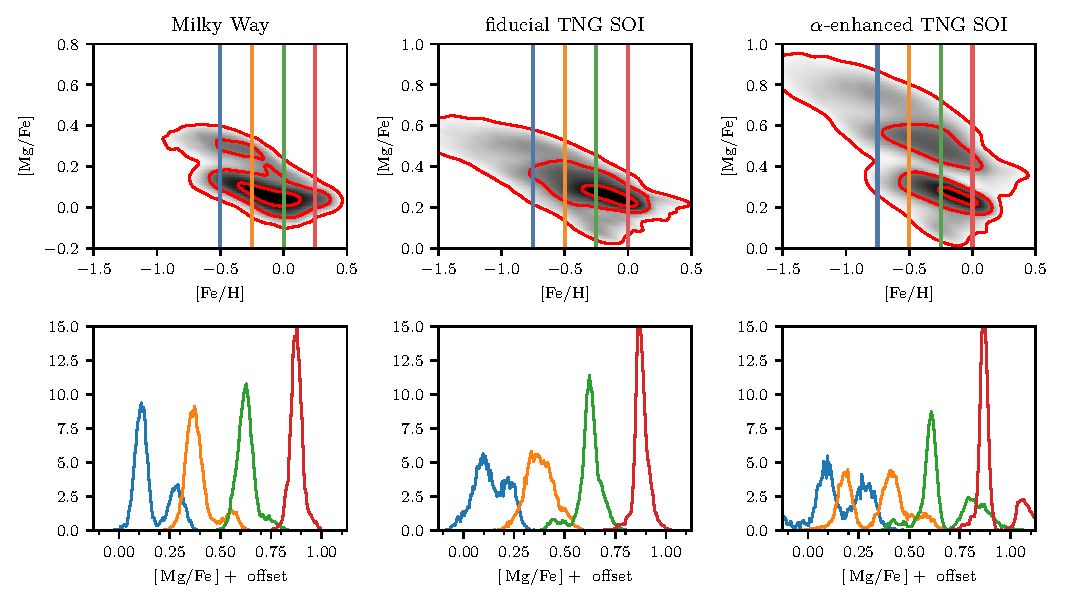
\includegraphics[width=\textwidth]{fig/392276.pdf}
  \caption{\textbf{When old stars are $\alpha$-enhanced, our subhalo of interest from TNG displays a prominent bimodality.} The upper left panel shows the distribution in the \MgFe{}-\FeH{} plane of the Milky Way, demonstrating a clear bimodality (data selection given in text). The lower left panel shows the 1D histograms of \MgFe{} at fixed \FeH{} values of $-0.5$, $-0.25$, $0$, and $0.25$ (blue, orange, green, and red, respectively). In the Milky Way, the bimodality is strongest at low metallicities while disappearing at high metallicities. The middle column shows the same plots but for our TNG subhalo of interest (392276) and with the fixed \FeH{} values $0.25\,\dex$ lower. No clear bimodality is detected at any metallicity. The right column shows the same subhalo but after increasing the \MgFe{} value of star particles formed before $z=1.5$ linearly with formation time (specifically by incrementing \MgFe{} by $0.1\times\left(t_{1.5}-t_{\textrm{form}}\right)$ if $t_{\textrm{form}} < t_{1.5}$, where $t_{1.5}$ is the age of the universe at $z=1.5$). A clear bimodality is shown in these panels which, unlike in the Milky Way, is present at all metallicities.}
  \label{fig:fig1}
\end{figure*}

\begin{figure*}
  \centering
  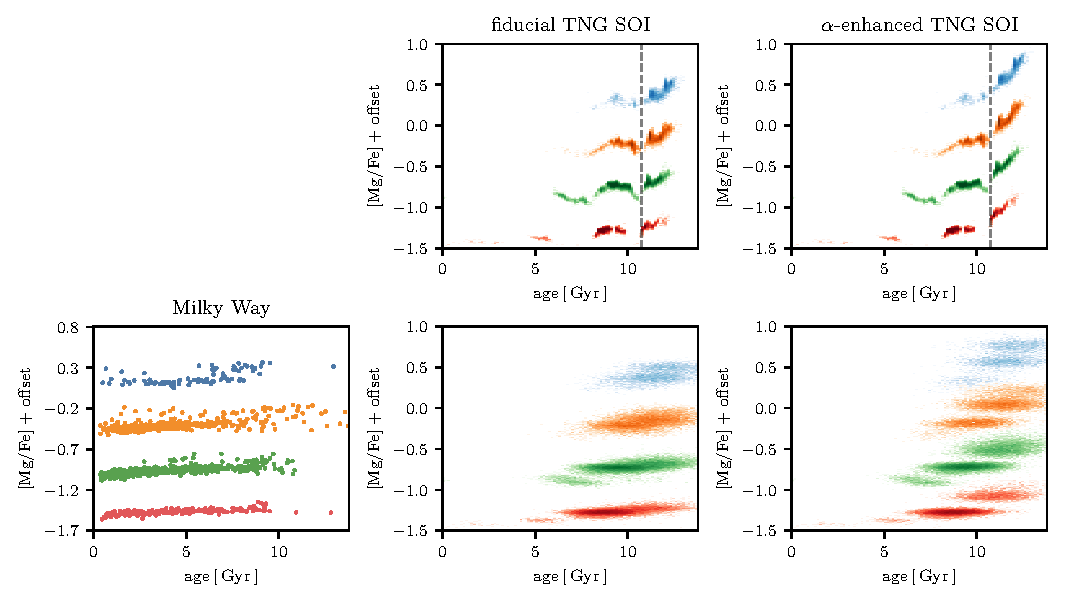
\includegraphics[width=\textwidth]{fig/392276_alpha.pdf}
  \caption{\textbf{Bimodality in the abundance plane is linked to distinct epochs in simulation.} The upper panels show \MgFe{} as a function of age for our subhalo in TNG. The colors indicate stellar populations at fixed values of \FeH{}, which are the same as in Figure~\ref{fig:fig1}. A gap in the relation occurs at an age of approximately $10.75\,\Gyr$, which we indicate with a vertical dashed line. The effect of the $\alpha$-enhancement is clear, as it more clearly separates the stars that form before and after this gap in ages (star particles which formed before $z=1.5$ are $\alpha$-enhanced, which occurs at an age of $\sim9.5\,\Gyr$). The lower panels show on the left the Milky Way and on the center and right the data from TNG but with $10\%$ age errors and $0.01\,\dex$ errors in \MgFe{}. When the simulations are given these errors, we see that the before and after star particles smear such that the two populations significantly overlap in ages. This feature more closely resembles the Milky Way, which displays such populations where the bimodality is strongest -- $\FeH=-0.5$ (blue) and $-0.25$ (orange).}
  \label{fig:alpha}
\end{figure*}

\begin{figure}
  \centering
  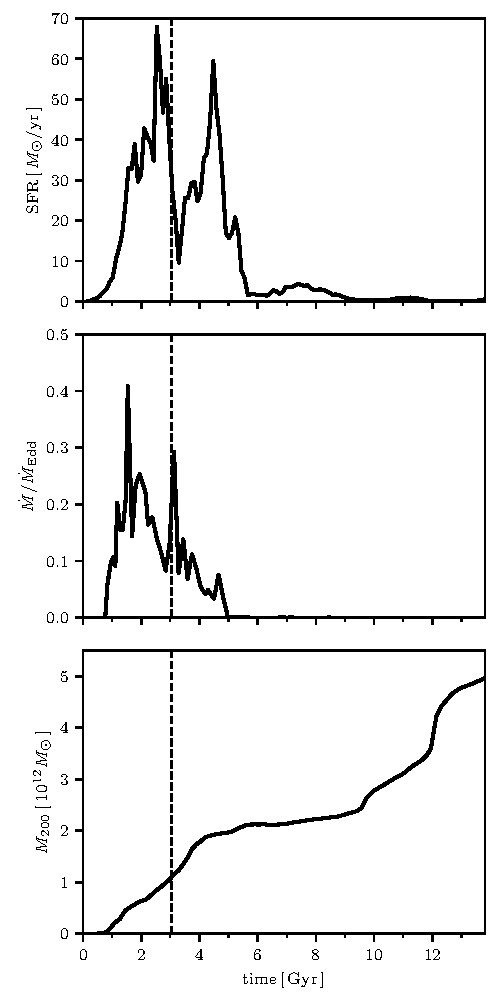
\includegraphics[width=\columnwidth]{fig/392276_SFH_AGN_M200.pdf}
  \caption{\textbf{The evolutionary history of our subhalo of interest.} The upper panel shows the SFH of our subhalo. This SFH is generated using the formation times of all star particles in the subhalo at $z=0$. In this and all subsequent panels we show a vertical dashed line at the same position as in Figure~\ref{fig:alpha}, which delineates the separation between the high- and low-$\alpha$ sequences. The gap in ages is naturally associated with a gap in the SFH located at the dashed line. The middle panel shows the BH accretion rate as a fraction of the maximum (Eddington) accretion rate across time. At early times the accretion rate is high, but the gap in ages is also coincident with a local spike in the accretion rate. In the lower panel we show the mass assembly of the halo, given as the mass within the radius that encloses $200\times$ the mean density of the universe. In this plot mergers are shown as sudden increases in the halo mass. Mergers at very early times when the halo is signifcantly less massive than its $z=0$ mass are not shown, but one can see that no clear merger is associated with the gap in stellar ages. Two mergers occur later on at $t\sim9$ and $\sim12\,\Gyr$.}
  \label{fig:history}
\end{figure}

\begin{figure}
  \centering
  \includegraphics[width=\columnwidth]{fig/mgfe_vice.pdf}
  \caption{\textbf{A higher star formation efficiency leads to a steeper decline in \MgFe{}.} In both panels, the lines show the time evolution of \MgFe{} in a simple one zone chemical evolution model, described in the text. The upper panel shows the evolution over $2\,\Gyr$ of \MgFe{} while the lower panel shows the negative of its time derivative. Decreasing the star formation timescale $\tau_{\star}=M_{\textrm{gas}/\textrm{SFR}}$ leads to a more rapid decline in \MgFe{}. At its steepest decline ($t\sim0.5\,\Gyr$), an order of magnitude decrease in $\tau_{\star}$ leads to a slope nearly a factor of $2$ larger. At later times ($t>1\,\Gyr$), the models with smaller $\tau_{\star}$ reach their steady-state \MgFe{} value more quickly.}
  \label{fig:vice}
\end{figure}

The main result of our paper is given in Figure~\ref{fig:fig1}. Here, we compare the abundance plane in the Milky Way (left column) to that in our subhalo of interest (middle column). The colored vertical lines show 1D conditional histograms at $\FeH=-0.75$, $-0.5$, $-0.25$, and $0$ \red{check}. The Milky Way shows a clear bimodal population, with a high-$\alpha$ sequence most clearly distinct from the low-$\alpha$ sequence at low metallicity. The two sequences merge around solar metallicity.

Our subhalo of interest, on the other hand, does not show a clearly bimodal structure in the fiducial simulation (middle column). There is some structure in the $\FeH=-0.75$ and $\FeH=0$ bins, but the peaks are close together ($<0.1\dex$) and the trough-to-peak ratio is high ($\sim1/2$ and $1/5$, respectively). It is not obvious that this distribution would have any structure with observational errors.

The right panel of Figure~\ref{fig:fig1} shows the same distribution as in the middle panel, but with an artificial declination in \MgFe{}. Star particles are given an additive offset of $0.1\times\left(t_{1.5}-t_{\textrm{form}}\right)$, where $t_{1.5}$ is the age of the universe at $z=1.5$ and $t_{\textrm{form}}$ is the formation time of the star particle. Only stars formed before $z=1.5$ are shown. Here, one can see a striking multimodal structure with three clear modes at $\MgFe\sim0.8$, $0.5$, and $0.2\,\dex$. These modes display more contrasted structure, with the distance between modes increasing (to $\sim0.2\,\dex$) as well as the trough-to-peak ratio decreasing to $\sim0.4$ between the $0.8$ and $0.5$ modes and practically vanishing between the $0.5$ and $0.2$ modes.

\subsection{Time Dependence}\label{sec:timedep}

\section{Discussion}\label{sec:disc}
In Figure~\ref{fig:fig1}, we compared the abundance plane between the Milky Way and our subhalo of interest. The result is quite simple, and indicates a fairly straightforward conclusion: multimodality is enhanced when \alphaFe{} more strongly declines with time. 

\subsection{Cause of $\alpha$ Decline}\label{ssec:sfe}
As discussed in Section~\ref{sec:intro}, it has long been known that the \alphaFe{} ratio should decline with time \red{cite}. This declination is caused by the relative enrichment contribution between Type II and Type Ia SNe, with the former contributing the bulk of the $\alpha$-elements and both contributing to Fe. However, this picture is complicated by the details of galaxy evolution. Inflows and outflows, radial gas transfer, and unmixed local enrichment all have a strong effect on the \alphaFe{} ratio.

A detailed accounting of all these processes is beyond the scope of this work, and much of it is impossible with the sparse snapshot spacing in TNG. However, we do offer one possible explanation for the relatively minor declination of \alphaFe{} in the simulation: the SFE at high surface densities in TNG is too low.

First, we demonstrate the impact of the SFE on the \alphaFe{} ratio using a simple one-zone chemical evolution model with the publicly available code \texttt{VICE}. The details of our setup is given in Section~\red{X}. We vary the star formation timescale, $\tau_{*}=M_{\textrm{gas}}/\textrm{SFR}$, and examine the impact on the \MgFe{} ratio asa function of time. We find that shorter star formation timescales lead to a more rapid reduction in \MgFe{}. A close match to our subhalo of interest in TNG is not attempted.

In TNG, the SF timescale is set to a fixed value of $2.2\,\Gyr$. However, this value is the SF timescale used to set the SFR of an individual cell. What is relevant for comparison to these models is the SF timescale averaged over some well-mixed region. 

\subsection{Full Sample}\label{ssec:fullsamp}

A version of Figure~\ref{fig:fig1} for the rest of the subhalos in our original sample are given in the Appendix. They display a variety of morphologies, likely arising from a similar variety of processes. They are the subject of continuing work.



\begin{acknowledgements}
This work has made use of data from the European Space Agency (ESA) mission {\it Gaia} (\url{https://www.cosmos.esa.int/gaia}), processed by the {\it Gaia} Data Processing and Analysis Consortium (DPAC, \url{https://www.cosmos.esa.int/web/gaia/dpac/consortium}). Funding for the DPAC has been provided by national institutions, in particular the institutions participating in the {\it Gaia} Multilateral Agreement.
\end{acknowledgements}

\bibliography{ref}{}
\bibliographystyle{aasjournal}

% \input{src/app.tex}

\end{document}
